\documentclass[11pt]{article}
\usepackage{geometry}                
\geometry{letterpaper}                   

\usepackage{graphicx}
\usepackage{amssymb}
\usepackage{epstopdf}
\usepackage[numbers]{natbib}
\usepackage{amssymb, amsmath ,empheq}
\DeclareGraphicsRule{.tif}{png}{.png}{`convert #1 `dirname #1`/`basename #1 .tif`.png}

\usepackage{listings}
\lstset{
basicstyle=\footnotesize,  
% keywordstyle=\color{blue},       		
  title=\lstname,  				
 numbers=left,                    			
 breakatwhitespace=false,
 breaklines=true
}

%\title{Title}
%\author{Name 1, Name 2}
%\date{date} 

\begin{document}



\thispagestyle{empty}

\begin{center}
\includegraphics[width=5cm]{ETHlogo.eps}

\bigskip


\bigskip


\bigskip


\LARGE{ 	Lecture with Computer Exercises:\\ }
\LARGE{ Modelling and Simulating Social Systems with MATLAB\\}

\bigskip

\bigskip

\small{Project Report}\\

\bigskip

\bigskip

\bigskip

\bigskip


\begin{tabular}{|c|}
\hline
\\
\textbf{\LARGE{Simulation of the Information Spreading}}\\
\textbf{\LARGE{in a Facebook Network}}\\
\\
\hline
\end{tabular}
\bigskip

\bigskip

\bigskip

\LARGE{Name 1 \& Name 2}



\bigskip

\bigskip

\bigskip

\bigskip

\bigskip

\bigskip

\bigskip

\bigskip

Zurich\\
December 2013\\

\end{center}



\newpage

%%%%%%%%%%%%%%%%%%%%%%%%%%%%%%%%%%%%%%%%%%%%%%%%%

\newpage
\section*{Agreement for free-download}
\bigskip


\bigskip


\large We hereby agree to make our source code for this project freely available for download from the web pages of the SOMS chair. Furthermore, we assure that all source code is written by ourselves and is not violating any copyright restrictions.

\begin{center}

\bigskip


\bigskip


\begin{tabular}{@{}p{4cm}@{}p{4cm}@{}@{}p{4cm}@{}}

\begin{minipage}{4cm}
\vspace{2cm}
\large Urs Lustenberger
\end{minipage}

&

\begin{minipage}{4cm}

\vspace{2cm}
 \large \hspace{4mm} Nino Wili

\end{minipage}

&

\begin{minipage}{4cm}
\vspace{2cm}
\large Patric Z\"ochbauer

\end{minipage}
\end{tabular}


\end{center}
\newpage

%%%%%%%%%%%%%%%%%%%%%%%%%%%%%%%%%%%%%%%



% IMPORTANT
% you MUST include the ETH declaration of originality here; it is available for download on the course website or at http://www.ethz.ch/faculty/exams/plagiarism/index_EN; it can be printed as pdf and should be filled out in handwriting


%%%%%%%%%% Table of content %%%%%%%%%%%%%%%%%

\tableofcontents

\newpage

%%%%%%%%%%%%%%%%%%%%%%%%%%%%%%%%%%%%%%%



\section{Abstract}

\section{Individual contributions}

\section{Introduction and Motivations}

\subsection{Introduction and fundamental questions}

Social Networks like facebook and twitter are growing very fast. Most young people like students do have an account in one ore more of them. Many articles, pictures and videos on the internet have a direct "share" button. It is a very interesting question how information spreads in such networks. First, the internet may have become the fastest and sometimes most important source of "news" and information beside the "traditional" media and second, companies seem to be very interested in "informing" the right people with their commercials. 
\\
\\
The simplest way to describe the information spreading uses similarities to epidemiology, which means that the flow of information of one person to another is looked at as an "infection". In this work, we implemented a simple model in a homogeneous way with a set of differential equations and their numeric solutions as well as an agent-based, heterogeneous model, using a real facebook network.
\\
The fundamental questions of this work are:

\begin{itemize}
\item Are there relevant differences in the time evolution of the homogeneous and the agent-based network?

\item Are there indiviuals which are more important to the spreading of information (also called influentials)? Can they be recognized in the sense of position and connectivity in the network?
\end{itemize}

\subsection{Motivation}

As the team of authors consists of two chemists and a mathematician, the personal motivations also have a broad range. We were glad to recognize the parallels between our simulations with statistical physics and chemical reaction kinetics... 
















\section{Description of the Model}

The process of information spreading has many similarities with epidemiology, therefore the well known SIR-model was adapted\cite{complexsystems}.  The ``susceptibles'', are not aware of the information and are called ``ignorants'' within this work. ``Infected'' individuals know about the information and are willing to share it with other people, in other words they spread it and are therefore called ``spreaders''. The adaptation of the epidemiological term ``recovered'' is not that straightforward as its meaning in this context is not entirely clear. However, they can be interpreted as individuals being aware of the information but do not share it with others. They are called "stiflers".
\\
\\
In the SIR-model as well as in the agent-based model, the following set of ``reaction equations'' was used (I: Ignorant, S: Spreader, R: Stifler):


\begin{empheq}[left=\empheqlbrace]{align}
& I + S \xrightarrow{\lambda} 2 S \\
& S + R \xrightarrow{\alpha} 2 R \\
& S + S \xrightarrow{\alpha} S + R 
\end{empheq}
\newline
The main difference to the standard SIR-model is that spreaders do not become stiflers spontaneously. This change is only induced by meeting another spreader or stifler.

\subsection{Homogeneous SIR model}

In the mathematical treatment of the homogeneous model, the set of differential equations is expressed in terms of the densities $i(t)=I(t)/N$, $s(t)=S(t)/N$ and $r(t)=R(t)/N$, where N is the number of individuals in the network.

\begin{empheq}[left=\empheqlbrace]{align}
& \frac{\text{d}i(t)}{\text{d}t} = -\lambda \cdot s(t)i(t) \\
& \frac{\text{d}s(t)}{\text{d}t} = \lambda \cdot s(t)i(t) - \alpha \cdot s(t)[s(t)+r(t)] \\
& \frac{\text{d}r(t)}{\text{d}t} = \alpha \cdot s(t)[s(t)+r(t)]
\end{empheq}



\subsection{Agent-based model}

In the inhomogeneous, agent-based model the individuals are connected in a certain manner (facebook friends in this particular work). Only connected agents are able to meet. If a meeting occurs, transitions are induced at a certain probability depending on the relation between the agents (details are discussed later). Additional to the different connectivity of the agents, they also have a different activity, i.e. different probability to meet somebody. 
\\
\\
To convert the reaction equations into an agent-based model, time was discretized and in each time step a series of two steps is performed. First, the agents randomly meet another agent they know or nobody. Only two-agent meetings are possible. In the second step, the status of the agents change corresponding to the situation. There are six possible combinations of ignorants, spreaders and stiflers. Three of them correspond to the ``reactions'' 1-3, the other ones (I+I, I+R and R+R) have no other influence than ``occupying'' the agents. The probability $\lambda$ was chosen to be dependent on the number of common friends. For simplicity, $\alpha$ was a constant.


\section{Implementation}

\subsection{The Network}
how did we get the network?

how did we get the coordinates with gephi?

\subsection{Homogeneous SIR-model}

Urs

\subsection{Agent-based model}

\subsubsection{Initial condition}

At the beginning of each simulation, all agents are ignorant but one, which is a spreader. This agent was determined pseudo-randomly.

\subsubsection{Determine the meetings}

(See \texttt{talkstep.m} for details.)
\newline
\newline
In order to determine who meets who, the program goes through the vector of agents (1:N) randomly (line 14-16). With a probability corresponding to the activity of that agent, he may meet somebody (line 19). The person he meets is determined randomly and must be one he knows and one which is not already meeting another agent in this time step (line 30 ). In order to be able to implement that agents with more friends meet more people and to keep the simple data structure first a random person is chosen out of all the persons in the network and after that, the program checks whether they know. Like that, lot of "finding attempts" land on pairs which are not connected, that's why more than one attempt is performed each round (line 22-39). \texttt{attempt} is basically just a scaling factor. Tests show that the number of meetings is still proportional to the product \texttt{activity * number of friends}.

\subsection{Status changes in meetings}




\section{Simulation Results and Discussion}

\subsection{Influentials}

\subsubsection{Existance and importance of influentials}


To analyise the existence of influentials, we first need to define its meaning. We will use de definiton given by Watts \cite{influentials}, which simply says that a person's importance is determined by the number of its \text{cumulative infections} (called casced).

\begin{figure}
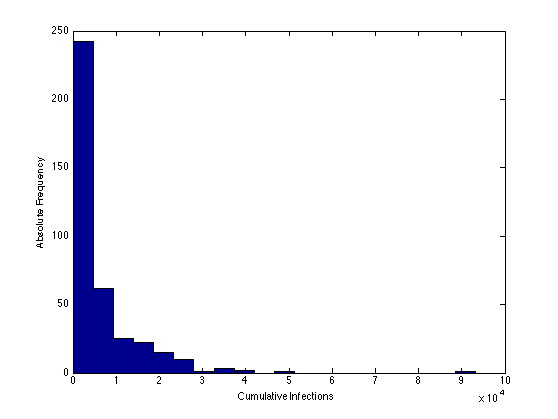
\includegraphics[width=7cm]{influ2}
\caption{sdlhfa}
\label{Histo}
\end{figure}

\begin{figure}
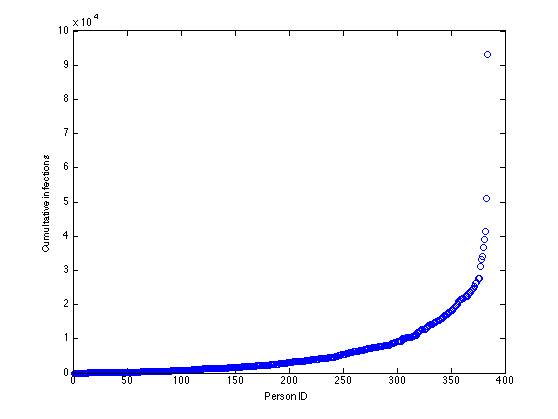
\includegraphics[width=7cm]{influ1}
\caption{sdlhfa}
\label{Sorted}
\end{figure}

Figure \ref{Histo} is a simple histogramm, that shows that the vast majority of people has only a small cumulative infection value. Whereas we see in Figure \ref{sorted} (which again plots the cumultative infection, sorted from small to large), that there are some (eventough only a few) with a very large cumultative infection value. \\

We can even go one step further and try to estimate the importance of those influentials on all infections that occur in total. In order to do so, we sort the people after their importance (defined as above). We then calculate the amout of infections conditioned that only the m least important person have been involved in the spreading process (1 $\le$ m $\le$ 384).\\
For instance, $m=384$ implies all infections that occured, when only the last (therefore most important) person has been excluded.\\
\\
Given these results, we get that 94\% of all infections, happen in the runs where the 1\%-quantile of the most important people (in our case 4) have contributed (ie. were not excluced). This again indicates their importance.

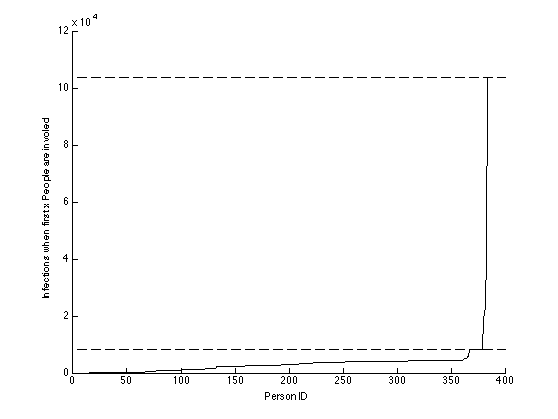
\includegraphics[width=7cm]{influ3}


According to Goldenberg \cite{word2mouth}, the importance of influential is often over-estimated. Our simulation strongly contradicts this statement. 

Reasons might be, that our networt is a) of relative small size and b) due to its construction we might overwighted some individuals (in particular, those with high number of mutualfriends)


\subsubsection{Determine influentials}

Obviously the next question that comes up, is the following. If we have influetials, how can we determine these in our network. Do they have properties that differs them from the other individuals? \\ 
\\
To find these mentioned, we have two possible aproaches: 
\\

1) Since our network is indeed a real world example of a Facebook Graph (the one of Patrick's Facebook Account). We can actually identify our, say top two, influetials. Then using this knowledge, we tried to narrow down the properties that might be of interest. 
It acutally turned out, that the two above mentioned induviduals indeed share very interessting propertiy. Namely, they are linkers of two or more cluster of our graph. 

2) Taking the results of 1) into consideration, it lead us to a more graph theroretical analysis of our data. Since we were interessted connectivity properties, we calculated the \textit{betweenness coefficent} for every node in our graph. 
It turns out that our top two influenctials indeed have the highest betweenness values. 

\begin{figure}
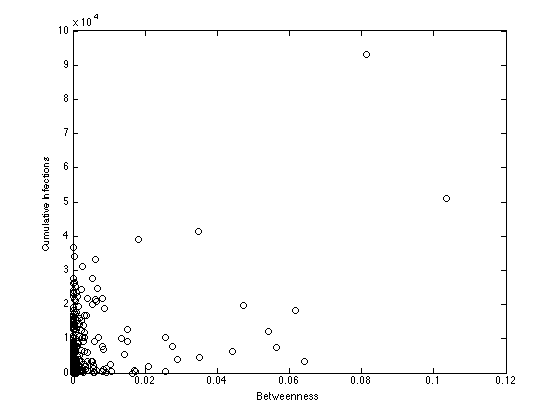
\includegraphics[width=7cm]{influ4}
\caption{sdlhfa}
\label{Betweenness}
\end{figure}

Figure \ref{Betweenness} shows, that high cumulative infection value implies high betweenness. But as we can also see in figure 3, it doesn't really imply the other direction.





\section{Summary and Outlook}

\begin{itemize}
\item Under certain circumstances the population profiles of the agent-based model differs significantly from those of the homogeneous model.
\item Individuals being more important for information spreading, in terms of cumulative infections, were found. The betweenness centrality might be used to roughly predict those especially influential individuals. 
\end{itemize}

\noindent Future work on this topic, should focus on getting more advanced data. Such that, the problems mentioned in section 6.1 can be avoided. Obviously, it would also be of interest to preform the experiment with more individuals. e.g. several connected networks. Further analysis can be done in the dependence of the parameters e.g. $\lambda$ on characteristics of the network. Also the parameter $\alpha$ could be investigated in more detail. 
Further on, to compare or even confirm the results, it would be desirable to gather real world data.

%%%%%%%%%%%

\section{Appendix}

\section*{Code}


\lstinputlisting[breaklines=true, language=Matlab]{../../code/talkstep.m}

\lstinputlisting[breaklines=true, language=Matlab]{../../code/parameters.m}

\begin{thebibliography}{9}

\bibitem{complexsystems}{
	A. Barrat, M. Barthélemy, A. Vespignani.
\newblock Dynamical Processes on Complex Networks.
\newblock \textit{Cambridge University Press}
\newblock Chapter 10, pp. 216-241

}

\bibitem{influentials}{
	D.J.Watts, P.S.Dodds.
\newblock Influentials, Networks, and Public Opinion Formation.
\newblock \textit{Journal of Consumer Research}
\newblock Vol 34, No. 4 (December 2007), pp. 441-458
}
	


\end{thebibliography}

\section{Additional figures}

\begin{figure}
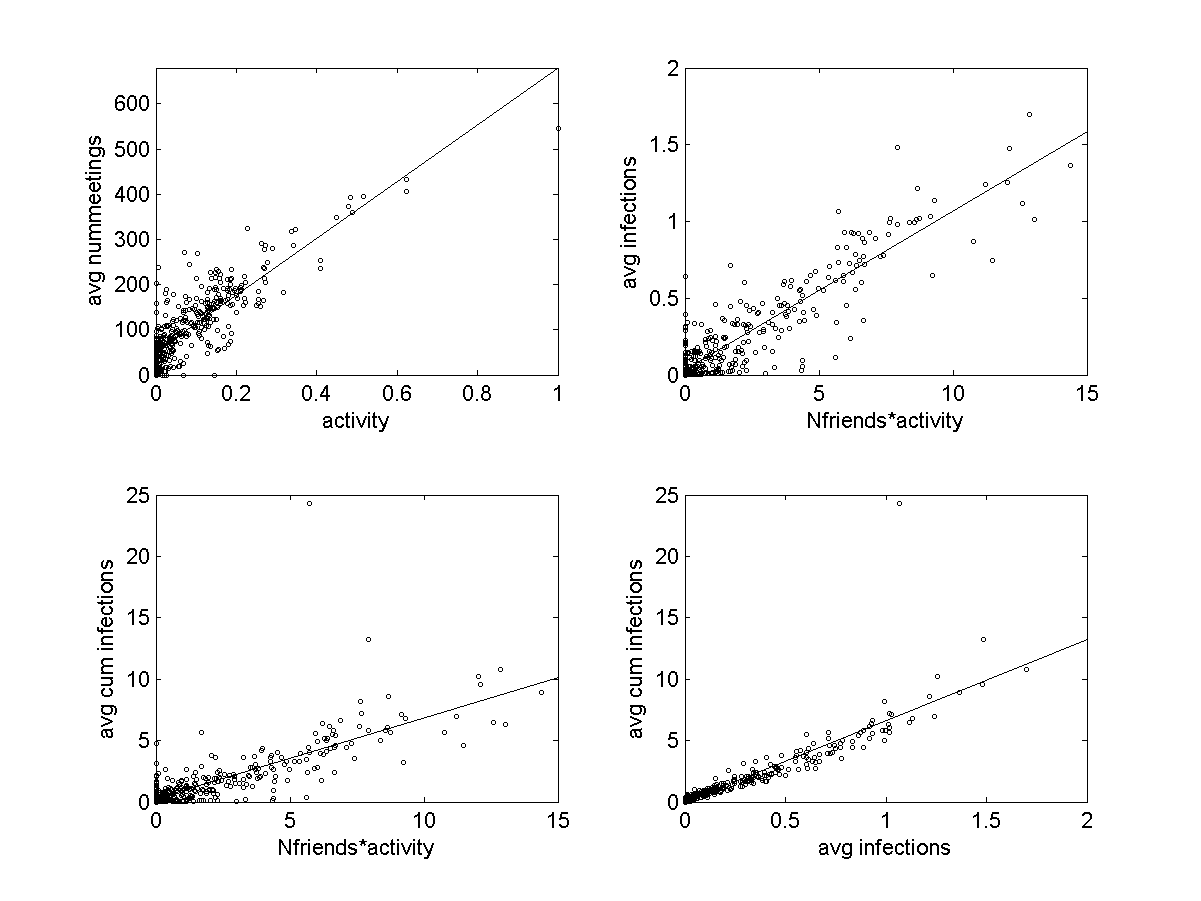
\includegraphics[width=7cm]{ImportantCorrelations}
\caption{sdlhfa}
\label{ImportantCorrelations}
\end{figure}

\begin{figure}
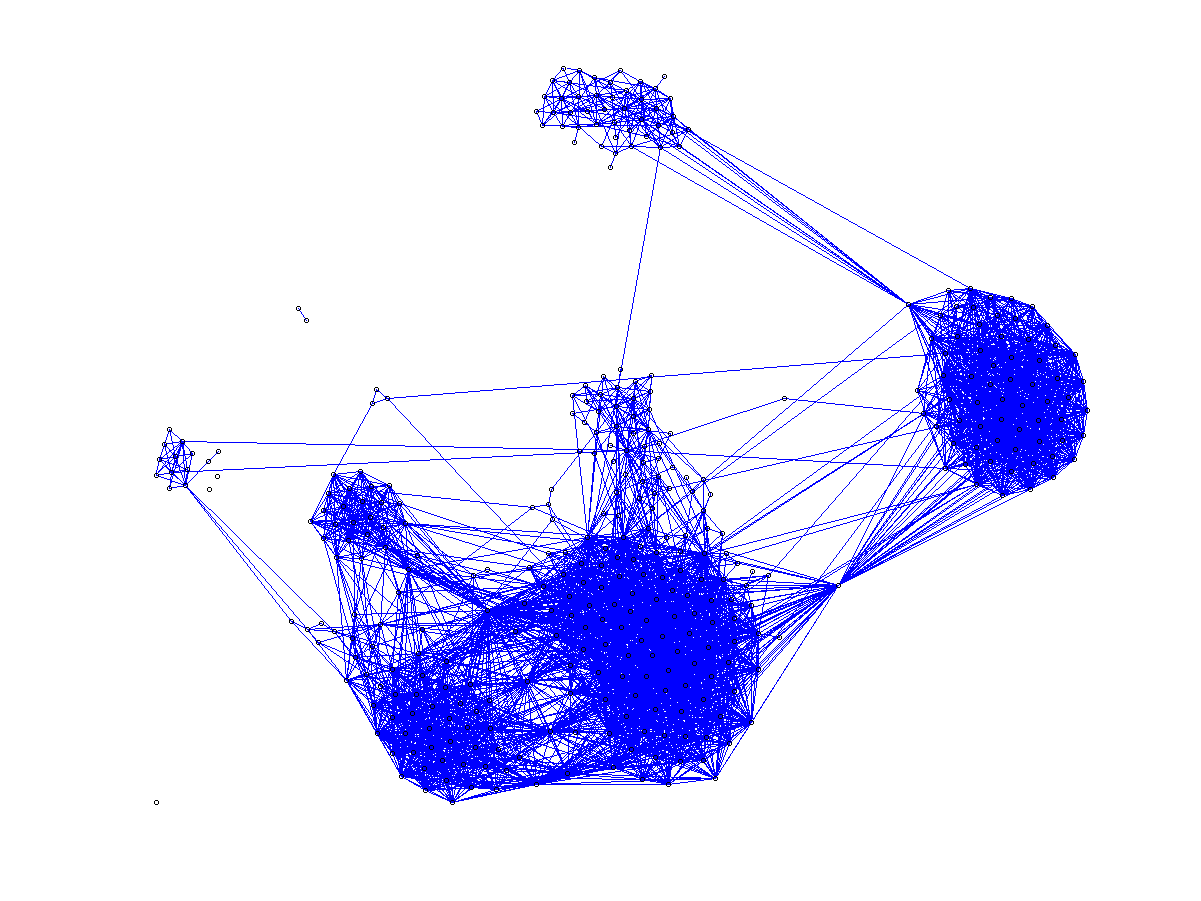
\includegraphics[width=7cm]{Network-Graph}
\caption{sdlhfa}
\label{Network-Graph}
\end{figure}





\end{document}  



 
